%
%  Chapter:  4 - Transverse Wobbling in 135Pr
%  Modified: 2/16/2015
%  Author:   James Till Matta
%
%%%%%%%%%%%%%%%%%%%%%%%%%%%%%%%%%%%%%%%%%%%%%%%%%%%%%%%%%%

\chapter{TRANSVERSE WOBBLING IN $^{135}$Pr}
\label{chp:trw}
%As stated in chapter \ref{chp:intro} wobbling is the longest anticipated fingerprint of triaxiality. Bohr and Mottelson predicted its existence in 1969 in the first edition of the second volume of their book nuclear structure\cite{bohrMottelson2}. Despite this longstanding prediction of its existence, the first discovery of wobbling was in 2001 by \O{}deg\aa{}rd \emph{et al.} \cite{wobblingIn163Lu}. Prior to this work wobbling had only been seen in five nuclei confined to the $A\sim{}170$ region, $^{161,163,165,167}$Lu \cite{wobblingIn163Lu,wobblingIn161Lu,wobblingIn165Lu,wobblingIn167Lu} and $^{167}$Ta \cite{wobblingIn167Ta}.

%Wobbling is the harmonic vibration of a nucleus's principal axis about its angular momentum vector. In the body fixed or intrinsic frame, wobbling is the harmonic vibration of the nucleus's angular momentum vector about one of its principal axes. In the simple wobbling mode, the principal axis used as a reference is the intermediate axis. This intermediate axis has the largest moment of inertia (MOI) and absent anything else is the preferred axis of rotation. In the transverse wobbling the reference principal axis is either the short or long axes as they are the axes that a quasiparticle with primarily particle nature or hole nature will couple to respectively. This coupling forces the rotation and wobbling motion to occur about these axes, eventually though the motion will become unstable and the wobbling will collapse as the rotation realigns itself to a new vector in the plane between the intermediate axis and the original axis of rotation. The final mode, longitudinal wobbling occurs when the Coriolis force aligns the quasiparticle to the intermediate axis. As in the simple wobbling case the rotation and wobbling occurs about the intermediate axis.
Understanding of the wobbling mode in nuclei has evolved quickly over the last 15 years. Bohr and Mottelson first showed that a rotating nucleus with stable triaxially deformed could have its rotational angular momentum precess and nutate about the principal axis of a nucleus (in analogy to the classical asymmetric top) \cite{bohrMottelson2} quite some time ago. H. Schnack-Petersen \emph{et al.} suggested in 1995 that bands in $^{163,165}$Lu which are based on the $\pi{}(i_{13/2})$ configuration, occupied a triaxial superdeformed (TSD) minimum of the total routhian surface \cite{tsdLutetium}. Following this there was rash of wobbling discoveries in $^{161,163,165,167}$Lu from 2001 to 2005 \cite{wobblingIn163Lu,wobblingIn163LuTwoPhonon,wobblingIn165Lu,wobblingIn167Lu,wobblingIn161Lu}. Further searches conducted in the region on $^{171}$Ta \cite{wobbSearch171Ta}, $^{169}$Ta \cite{wobbSearch169Ta}, $^{163}$Tm \cite{wobbSearch163Tm}, $^{171,172}$Hf \cite{wobbSearch1712Hf}, and ${160,161}$Tm \cite{wobbSearch1601Tm} yielded no further wobbling bands. This left an open problem as to why wobbling was only appearing in the Lu isotopes.

A possible solution to this problem was offered up in the TAC calculations by S. Frauendorf presented in Ref. \cite{wobbSearch163Tm}. The calculations suggest that the Lu TSD minima have a low density of states, low enough that the relatively high excitation energy wobbling mode can be observed. Contrariwise, the TSD minima of other nuclei in the region had a high density of states which could produce many different TSD bands with alternate configurations at similar energies. Thus, it is not that wobbling is absent in nuclei that are not Lu isotopes, but instead, that outside of the Lu isoptopes there was a competition between wobbling and particle hole excitations that favored the latter. This result motivated a search of $^{167}$Ta for wobbling which, in 2009, yielded the first wobbling band outside the Lu isotopes.


\section{Previous Cases of Wobbling}
\label{sec:trw-prev}
One phonon wobbling was first observed in 2001 in the nucleus $^{163}$Lu by S.W. \O{}deg\aa{}rd \emph{et al.} \cite{wobblingIn163Lu}. In 2002 two phonon wobbling was observed in the same nucleus by D.R. Jensen \emph{et al.} \cite{wobblingIn163LuTwoPhonon} (partial level scheme pictured in the left panel of Fig. \ref{fig:chp4-first-wobb}). In 2003 one and two phonon wobbling was discovered in $^{165}$Lu by G. Sch\"onwa\ss{}er \emph{et al.} \cite{wobblingIn165Lu} (partial level scheme pictured in the right panel of Fig. \ref{fig:chp4-first-wobb}). Later that same year came the discovery of one phonon wobbling in $^{167}$Lu by H. Amro \emph{et al.} \cite{wobblingIn167Lu} (partial level scheme pictured in the left panel of Fig. \ref{fig:chp4-second-wobb}). 2005 was the year of the discovery of one phonon wobbling  $^{161}$Lu by P. Bringel \emph{et al.} \cite{wobblingIn161Lu} (partial level scheme pictured in the right panel of Fig. \ref{fig:chp4-second-wobb}). The last of the wobblers known prior to this work, $^{167}$Ta, was discovered in 2009 by D.J. Hartley \emph{et al.} \cite{wobblingIn167Ta} (partial level scheme pictured in Fig. \ref{fig:chp4-last-wobb}). 

\begin{figure}[ht!]
\centerline{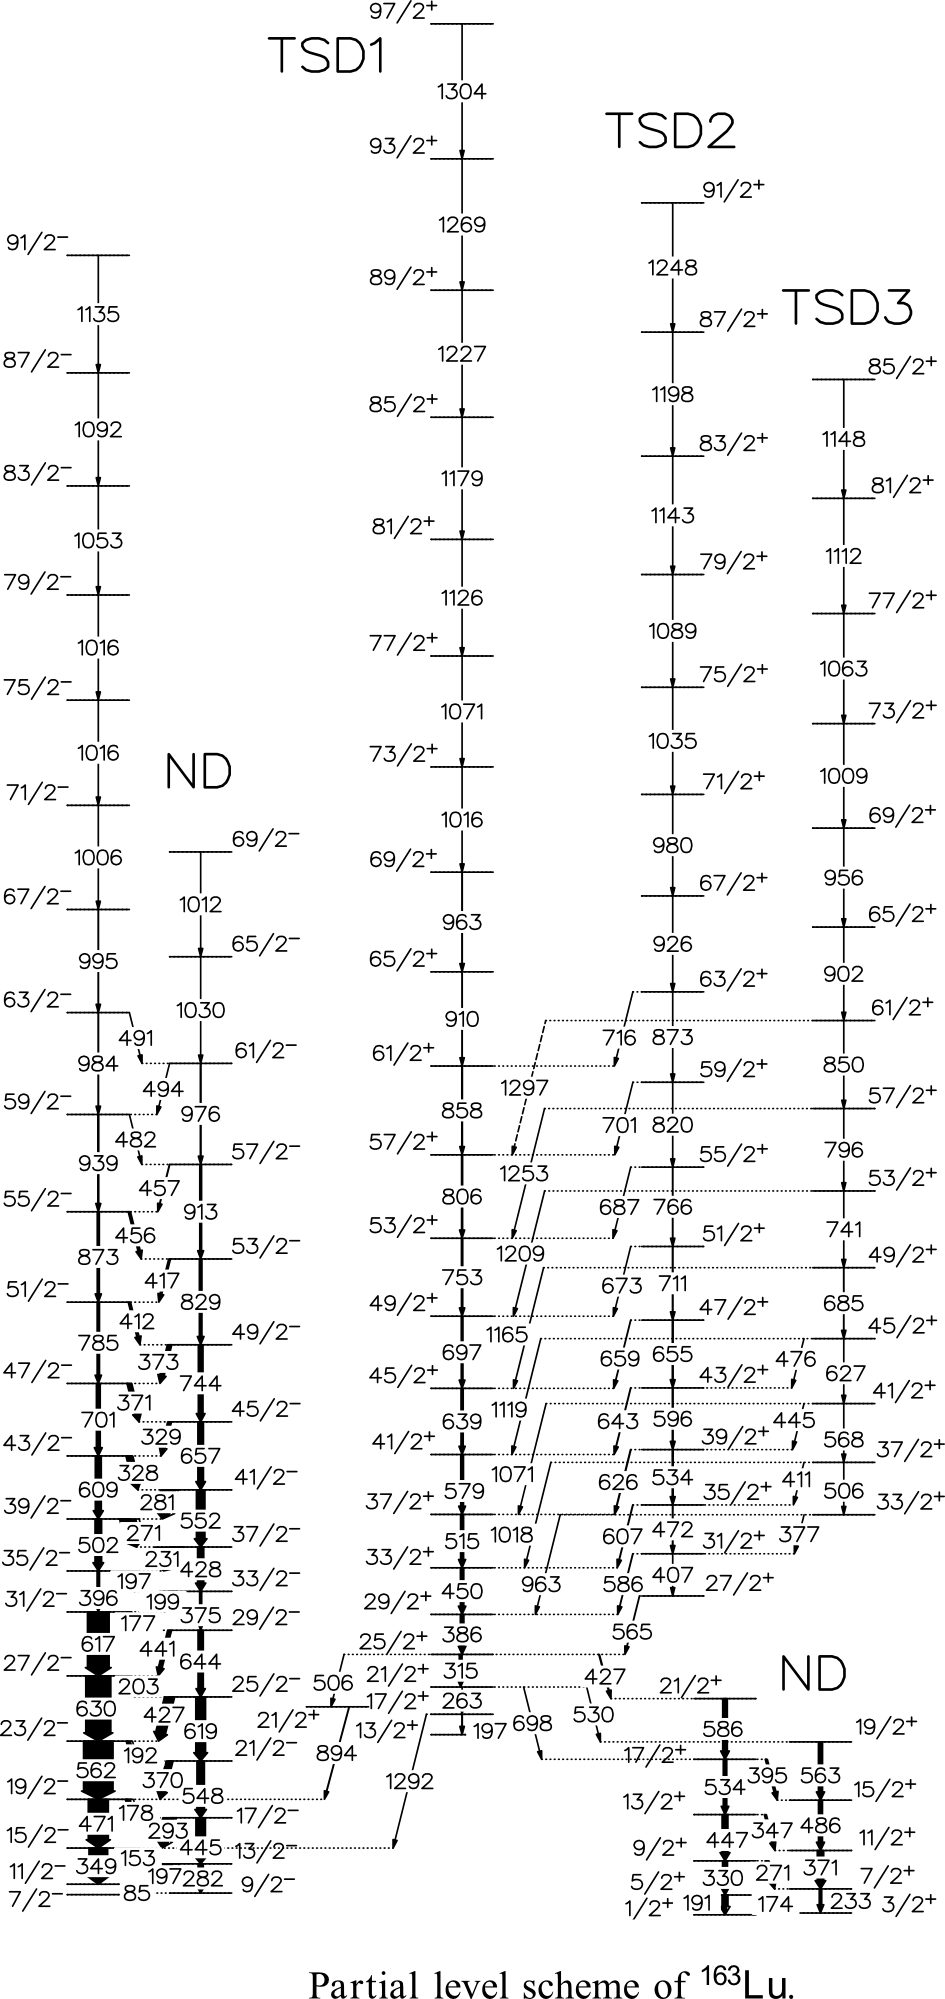
\includegraphics[width=0.4\textwidth]{./img/c4/163Lu_scheme.png}\hspace{0.1\textwidth}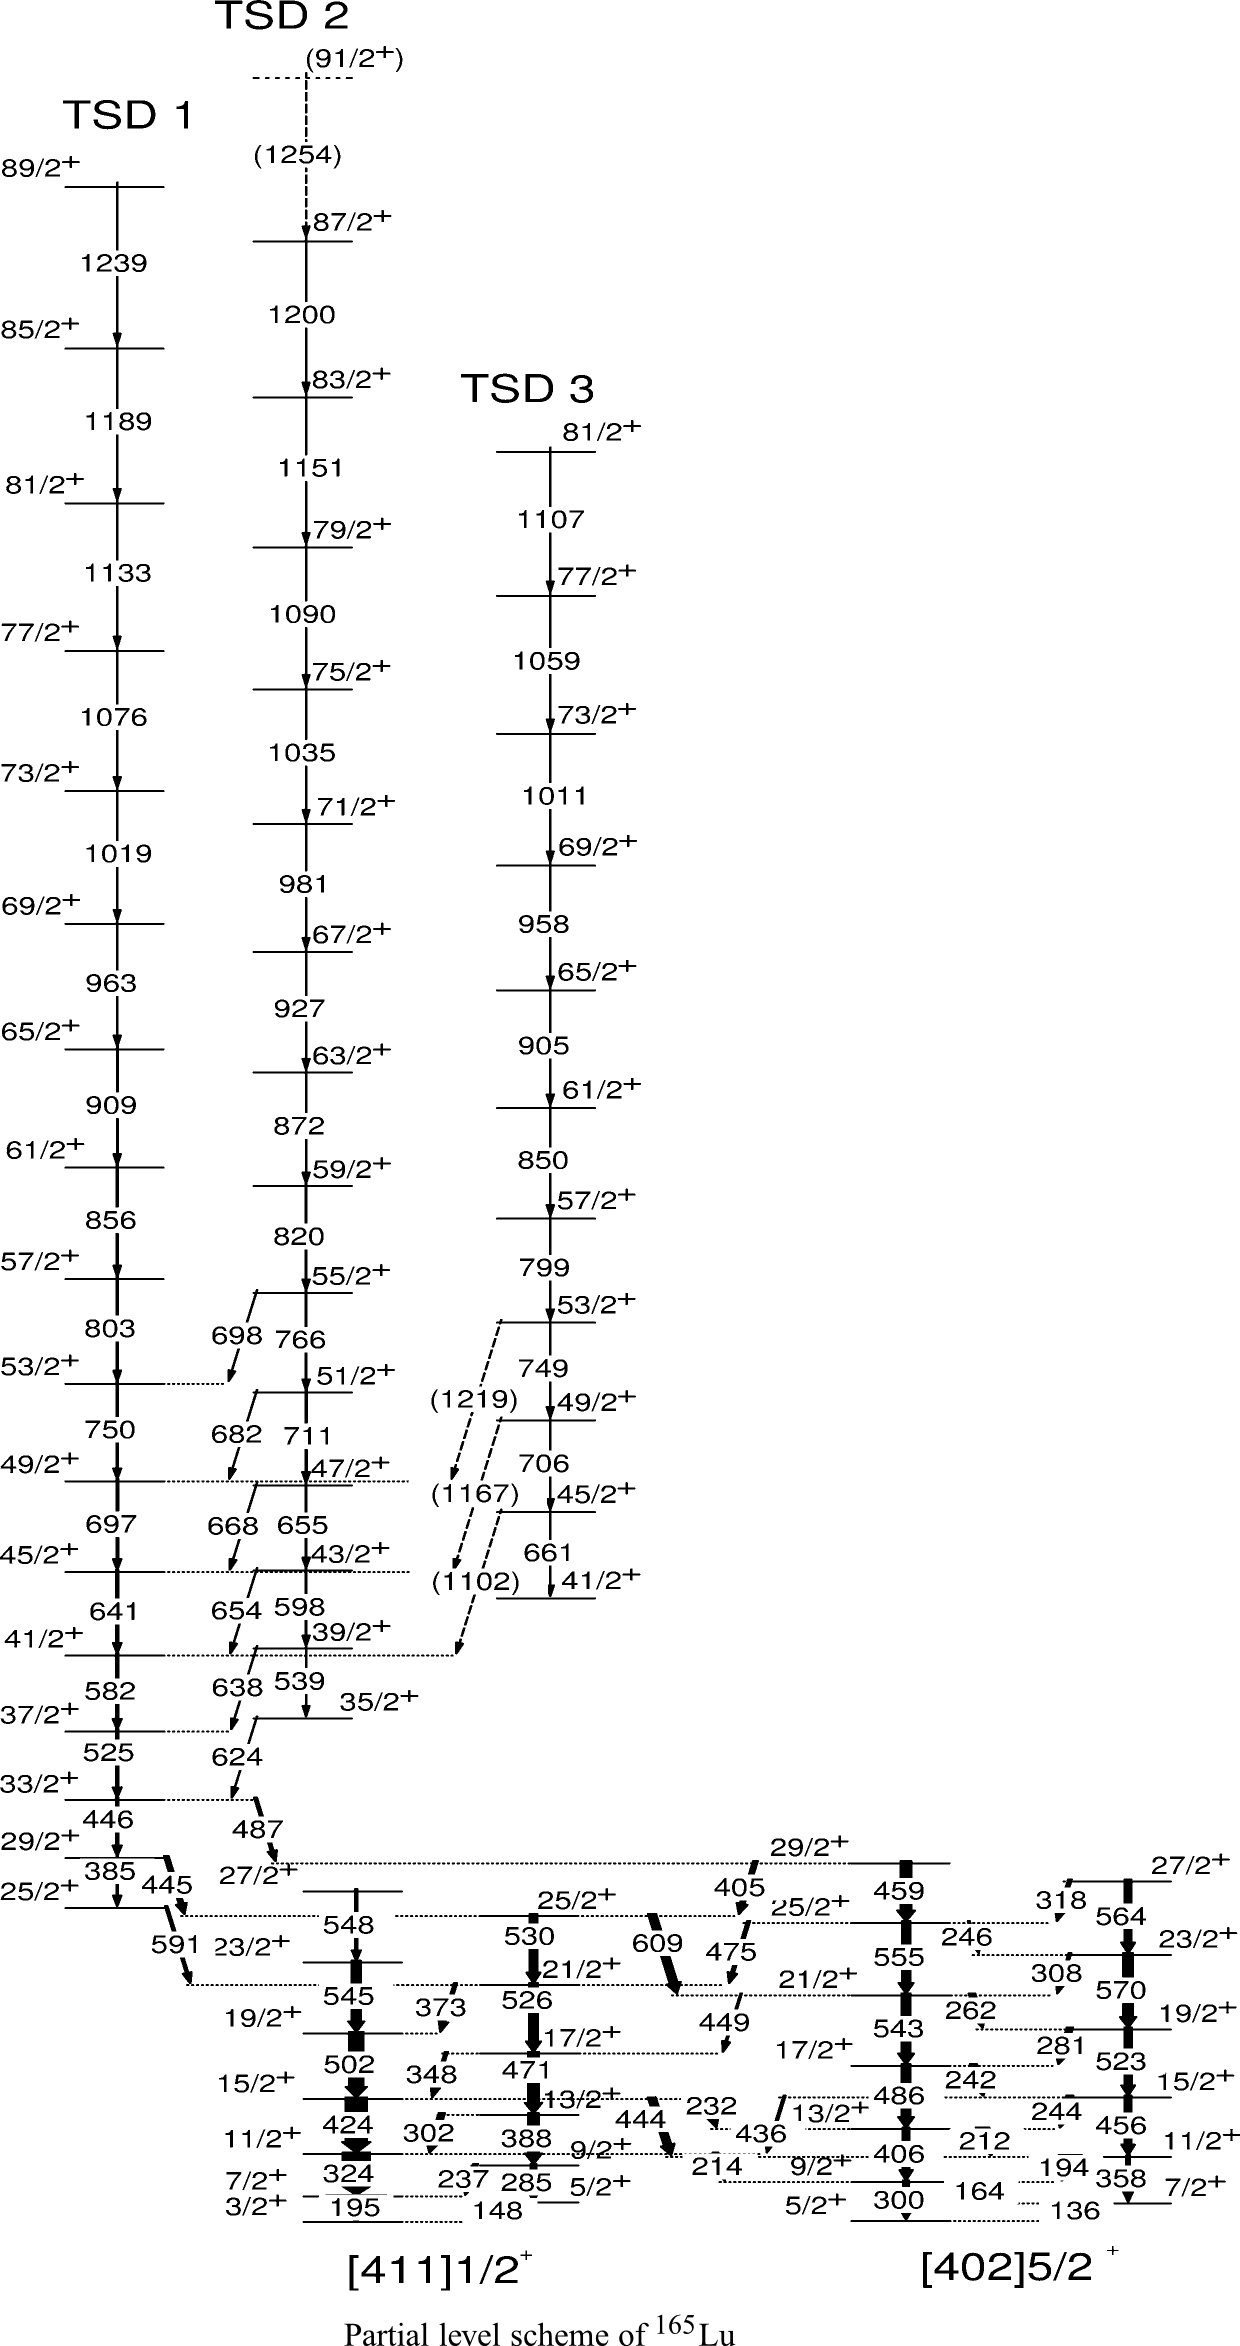
\includegraphics[width=0.4\textwidth]{./img/c4/165Lu_scheme.png}}
	\caption{Partial level schemes of $^{163}$Lu (left) and $^{165}$Lu (right). Figures adapted from Ref. \cite{wobblingIn163LuTwoPhonon} and Ref. \cite{wobblingIn165Lu} respectively. In $^{163}$Lu the $n_w=0,1,2$ bands are labeled TSD1, TSD2, and TSD3 respectively. In $^{165}$Lu the $n_w=0,1,2$ bands are labeled TSD1, TSD2, and TSD3 respectively.\label{fig:chp4-first-wobb}}
\end{figure}

\begin{figure}[ht!]
\centerline{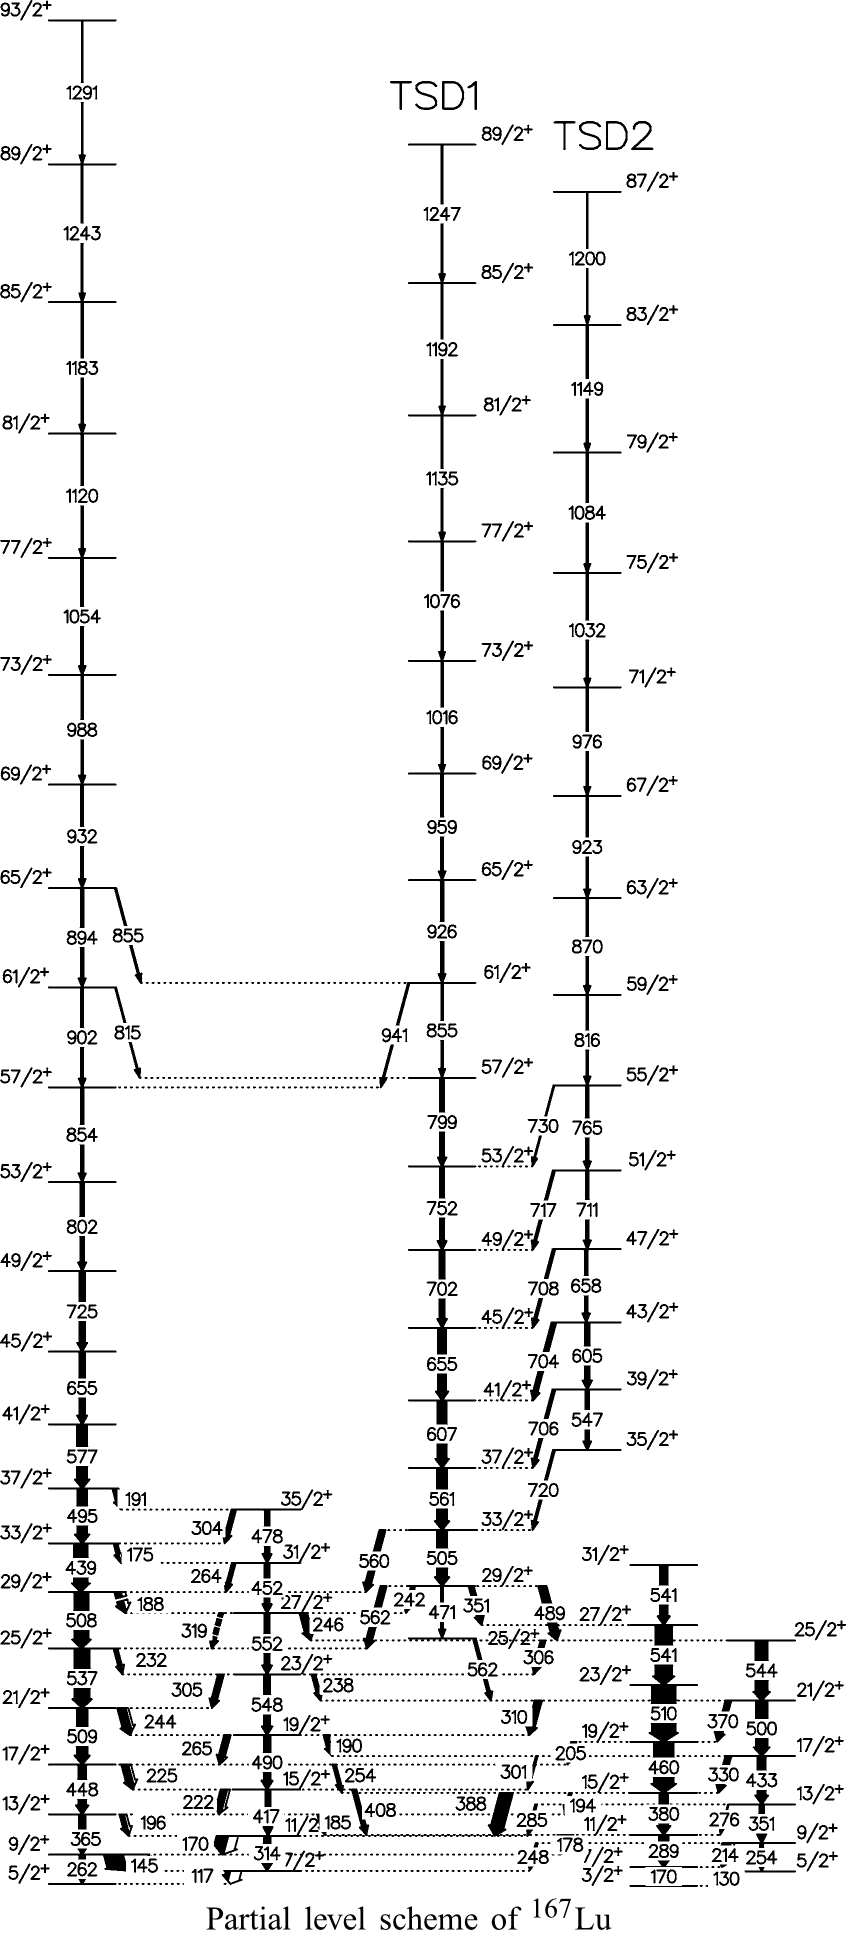
\includegraphics[width=0.4\textwidth]{./img/c4/167Lu_scheme.png}\hspace{0.1\textwidth}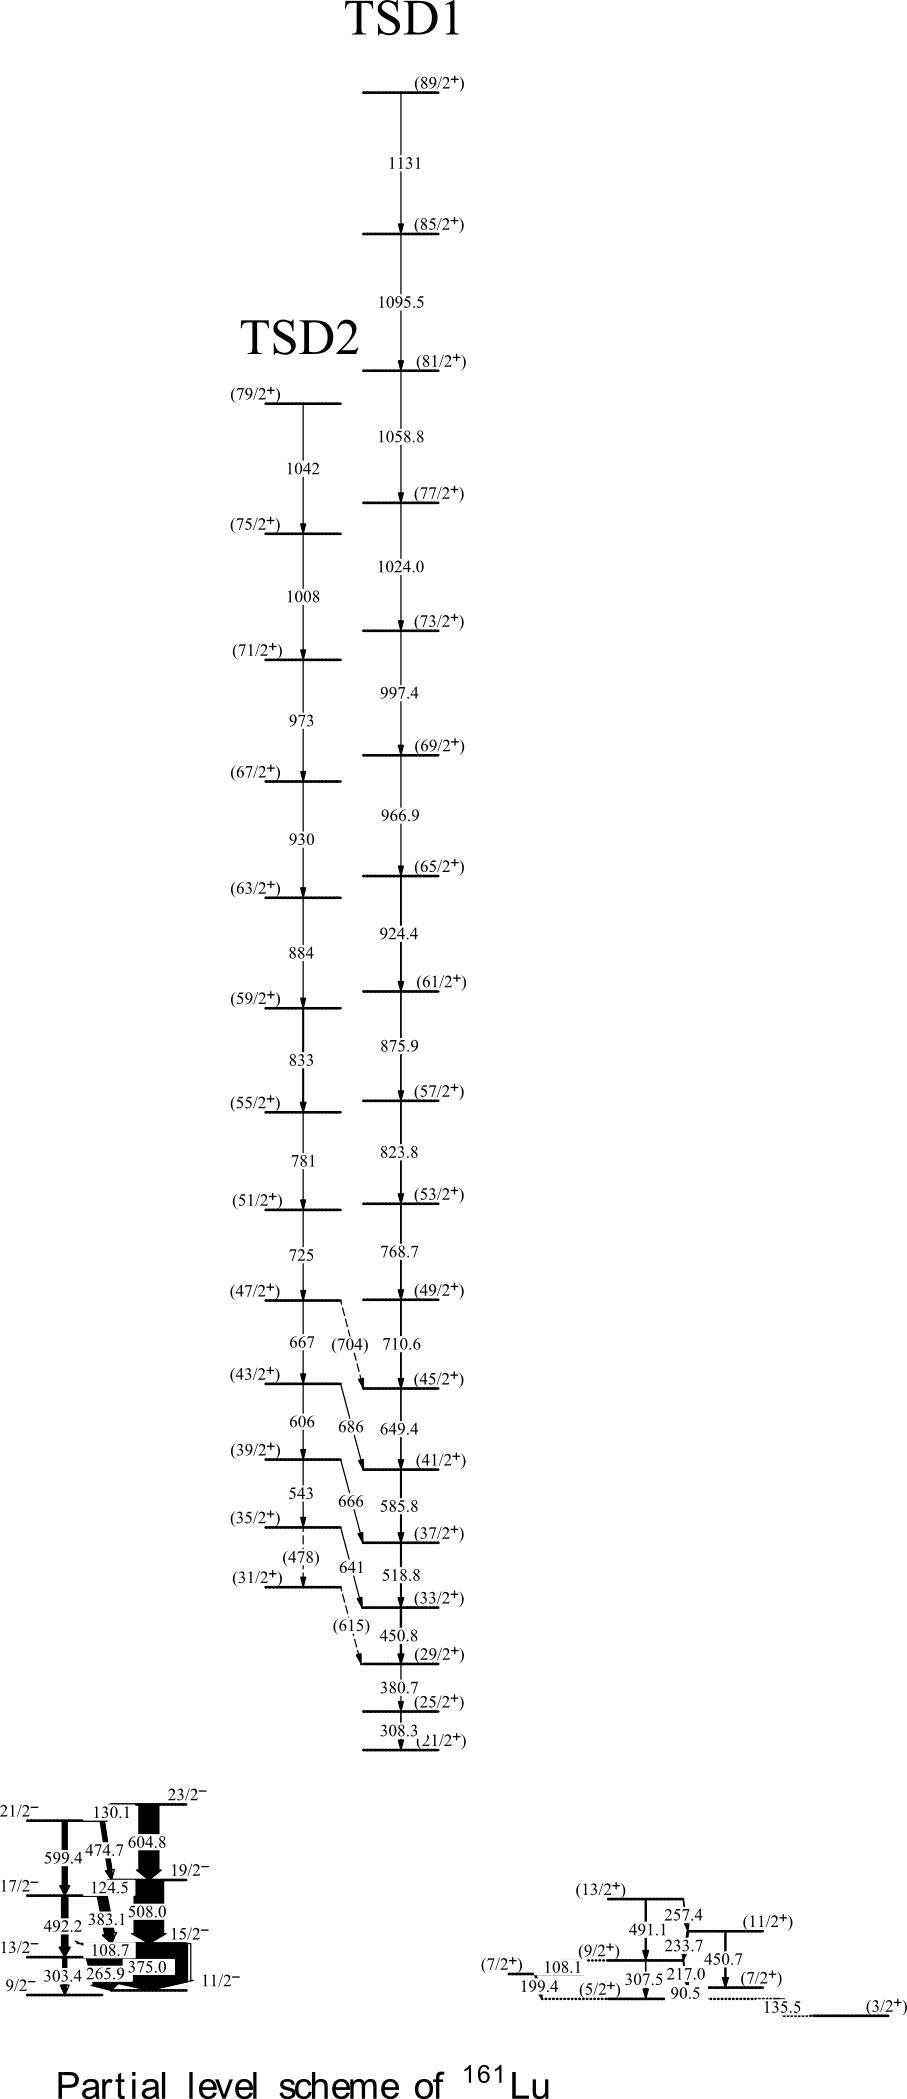
\includegraphics[width=0.4\textwidth]{./img/c4/161Lu_scheme.png}}
	\caption{Partial level schemes of $^{167}$Lu (left) and $^{161}$Lu (right). Figures adapted from Ref. \cite{wobblingIn167Lu} and Ref. \cite{wobblingIn161Lu} respectively. In $^{167}$Lu the $n_w=0,1$ bands are labeled TSD1 and TSD2 respectively. In $^{161}$Lu the $n_w=0,1$ bands are labeled TSD1 and TSD2 respectively.\label{fig:chp4-second-wobb}}
\end{figure}

\begin{figure}[ht!]
\centerline{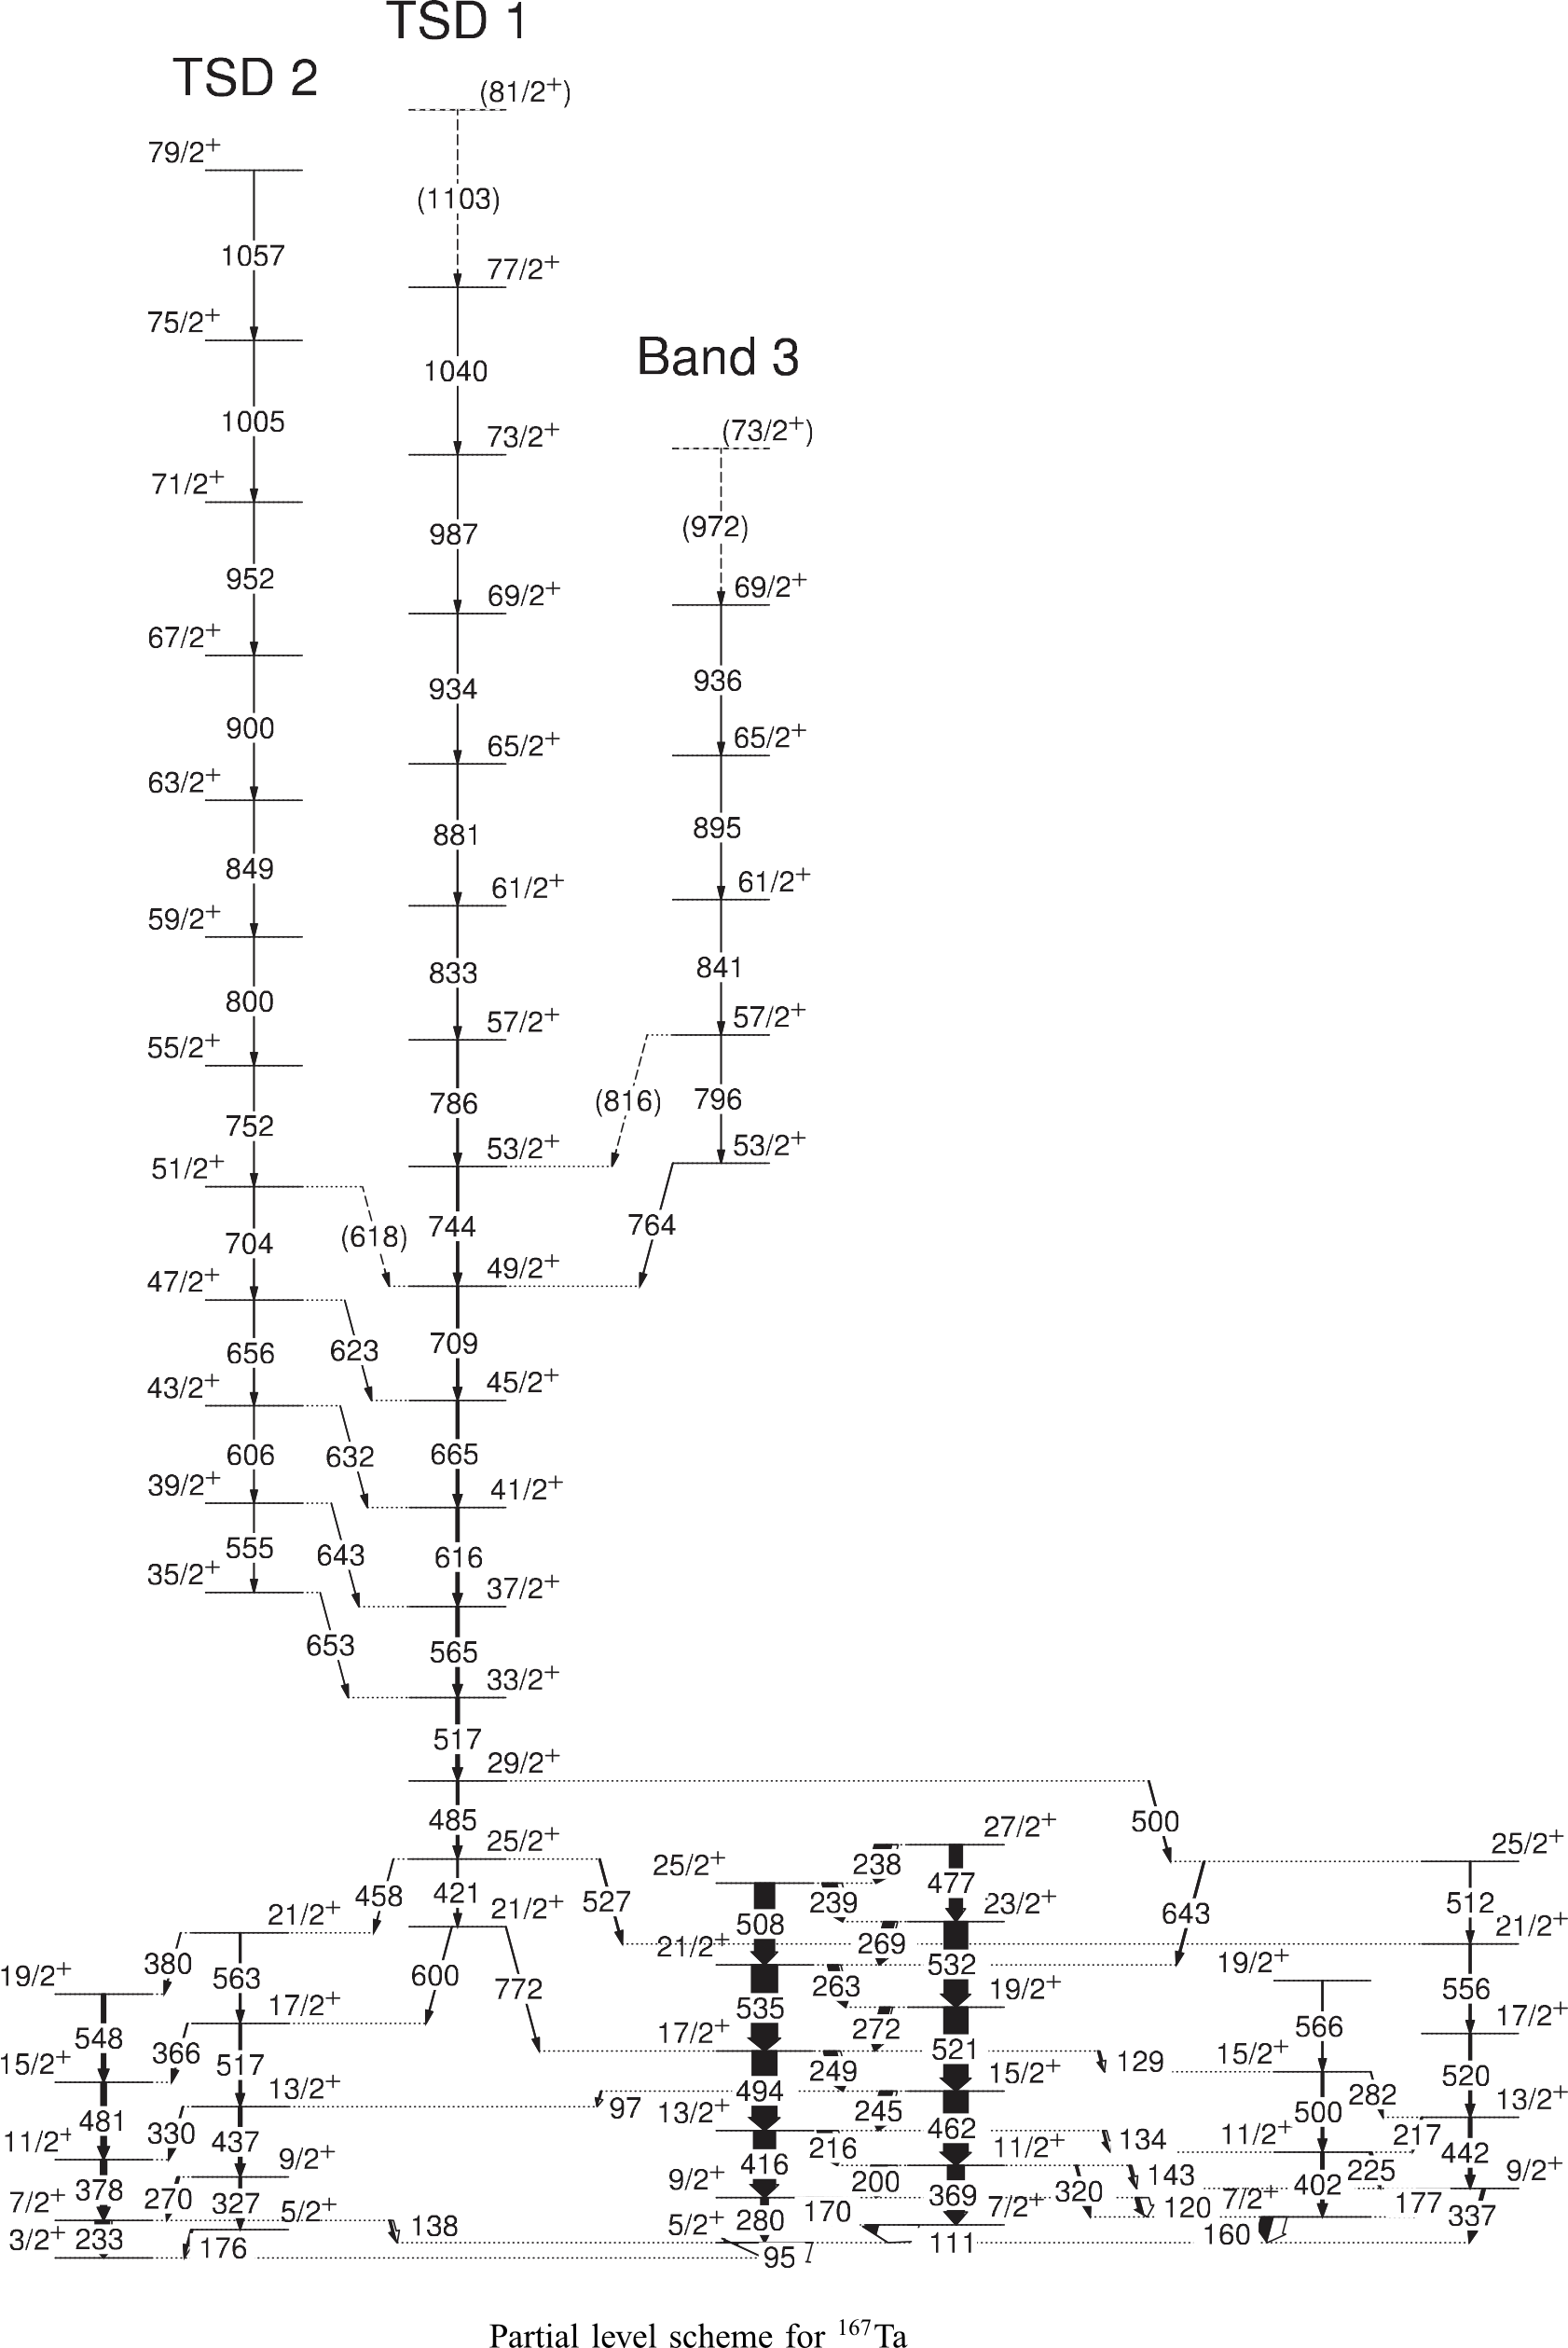
\includegraphics[width=0.4\textwidth]{./img/c4/167Ta_scheme.png}}
	\caption{Partial level scheme of $^{167}$Ta. Figure adapted from Ref. \cite{wobblingIn167Ta}. The $n_w=0,1$ bands are labeled TSD1 and TSD2 respectively.\label{fig:chp4-last-wobb}}
\end{figure}

Following the discovery of the first wobbling structure, calculations using the QTR model were used to describe the wobbling mode \cite{oldQTRWobblingTheory1,oldQTRWobblingTheory2,oldQTRWobblingTheory3,oldQTRWobblingTheory4}. Later, microscopic random phase approximation (RPA) calculations \cite{wobblingRPAMatsuzaki,wobblingRPAMatsuzaki2,wobblingRPAOi,wobblingRPAShimizu,wobblingRPAshoji} were used as well. Both theories do well in reproducing the large $B(E2)_{out}/B(E2)_{in}$ interband to intraband ratios seen in experiment. However, the QTR model, using the assumptions that the odd quasiparticle aligns with the intermediate axis \cite{oldQTRWobblingTheory1,oldQTRWobblingTheory2,oldQTRWobblingTheory3,oldQTRWobblingTheory4}, failing to reproduce the experimentally observed decrease in the wobbling energy (see Fig. \ref{fig:chp4-old-wobb-freq}) which is defined by:
\begin{equation}
\label{eqn:chp4-wobb-freq}
\Delta{}E=\hbar\omega_w(I)=E(I,n_w=1)-(E(I-1,n=0)+E(I+1,n_w=0))/2
\end{equation}
In constrast the microscopic RPA calculations were able to reproduce the observed decrease in wobbling energy.
\begin{figure}[ht!]
\centerline{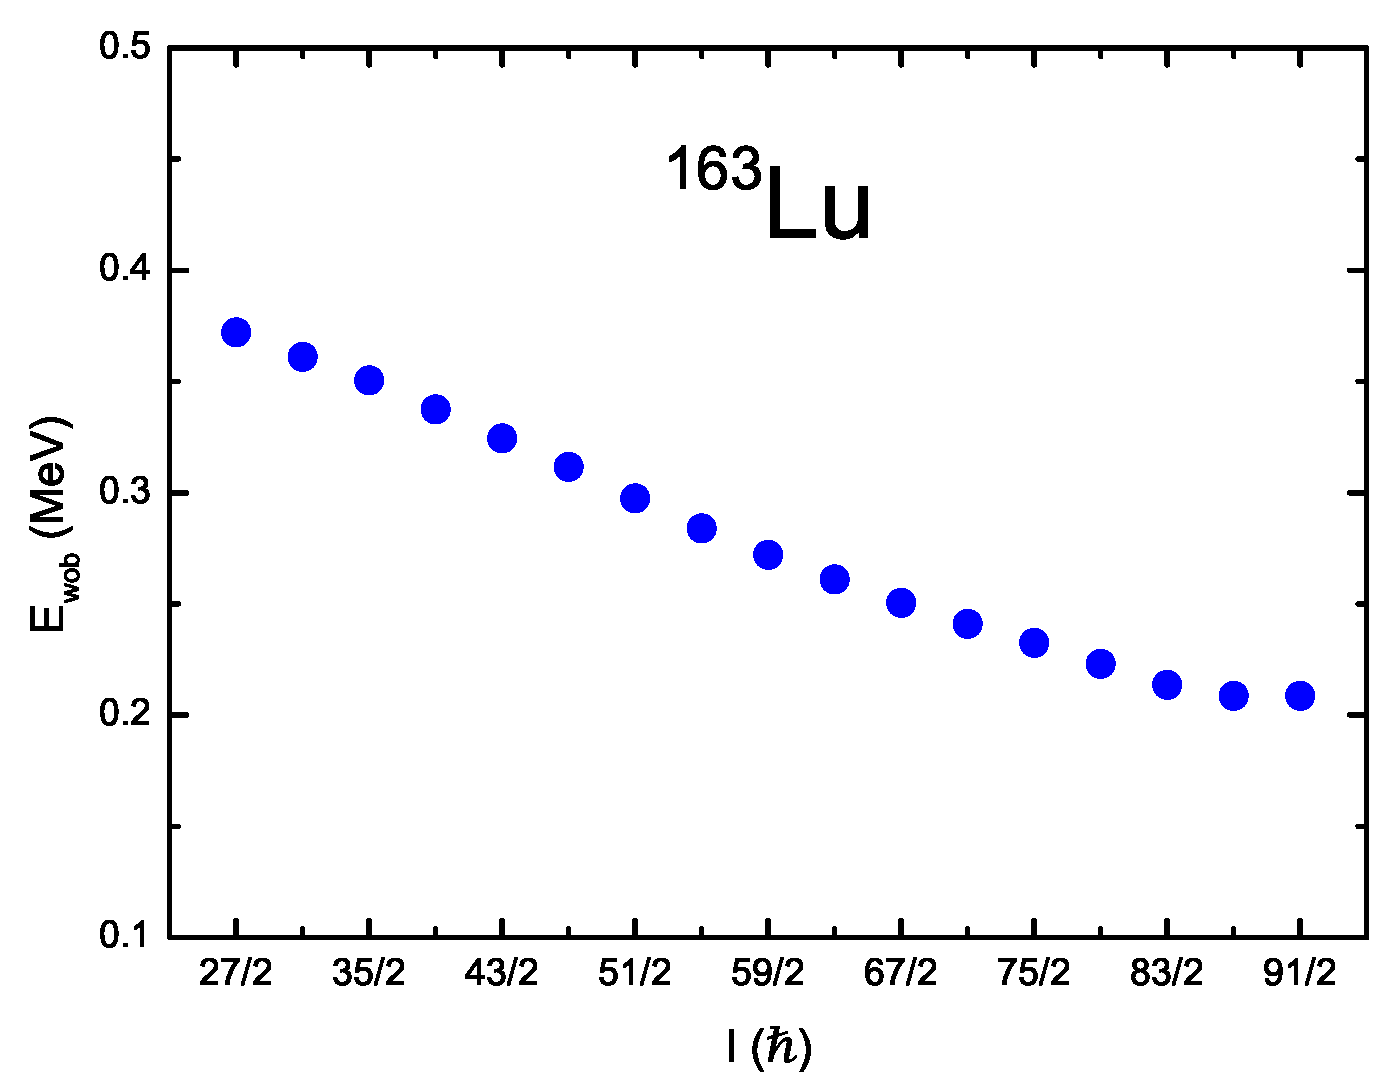
\includegraphics[height=0.25\textheight]{./img/c4/163Lu_plot.eps}\hspace{0.1\textwidth}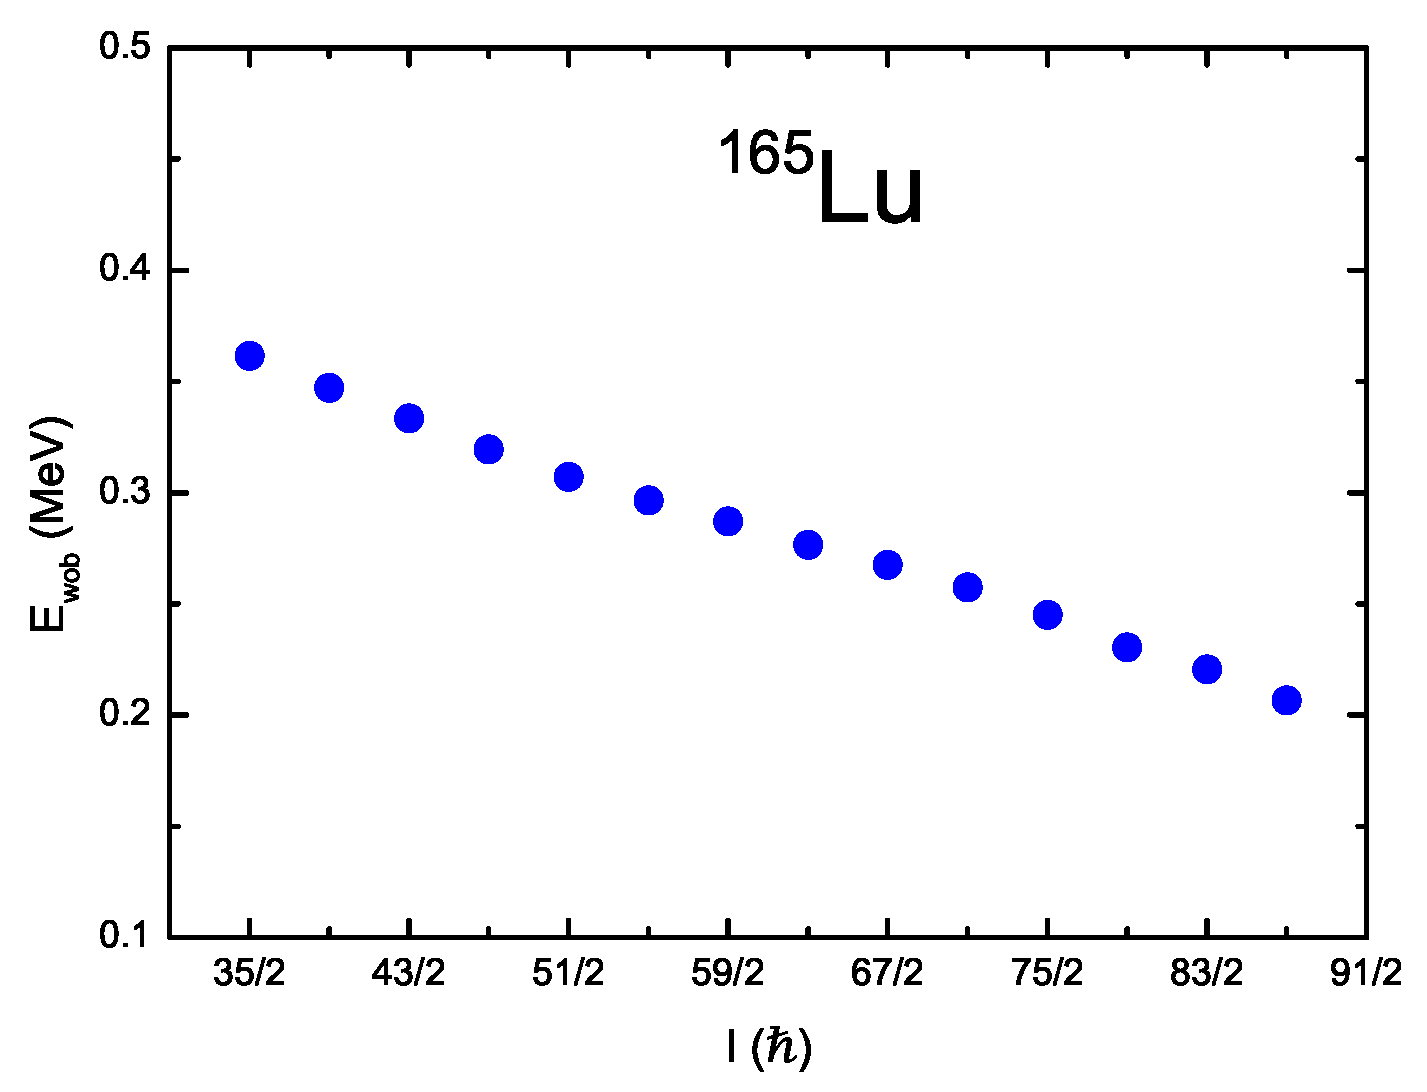
\includegraphics[height=0.25\textheight]{./img/c4/165Lu_plot.eps}}
\centerline{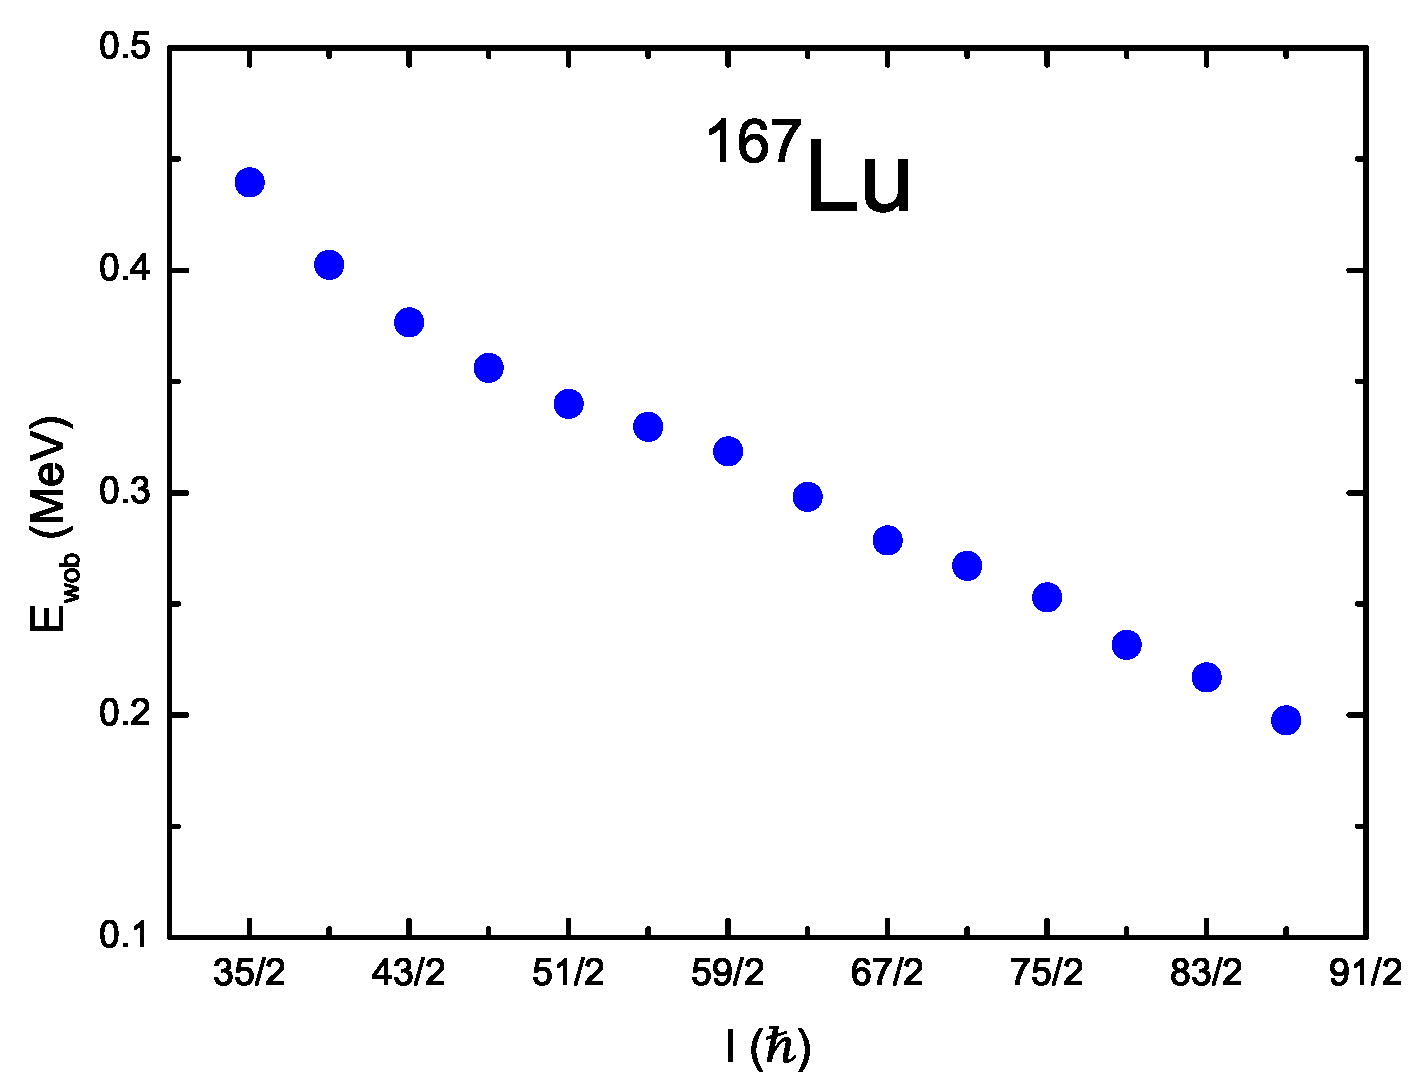
\includegraphics[height=0.25\textheight]{./img/c4/167Lu_plot.eps}\hspace{0.1\textwidth}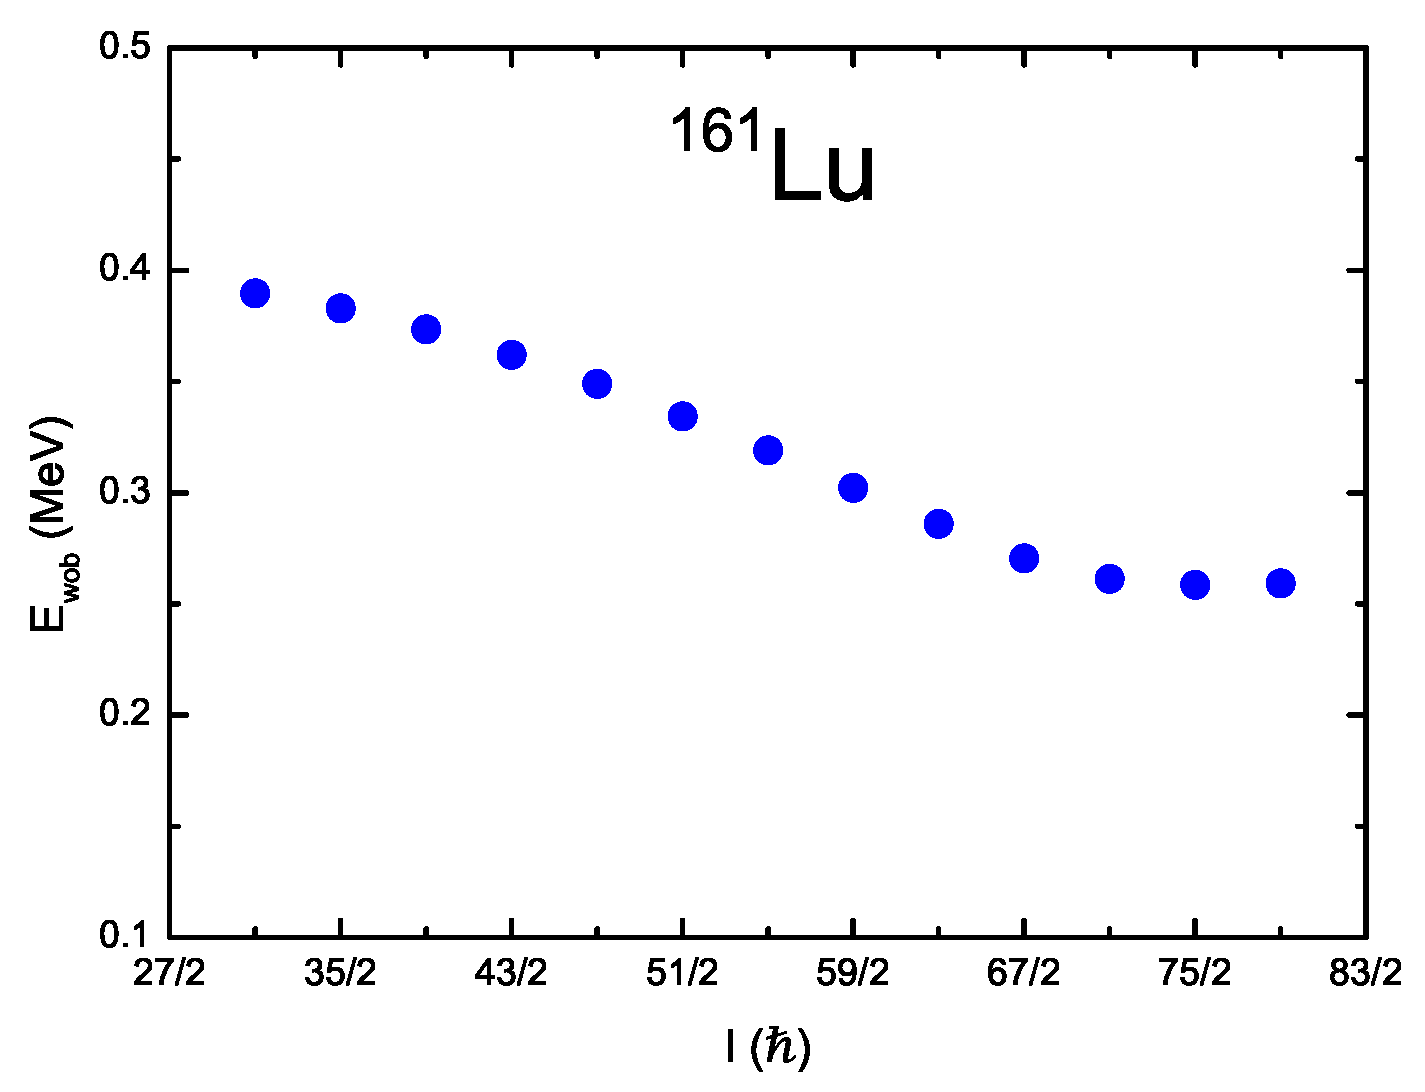
\includegraphics[height=0.25\textheight]{./img/c4/161Lu_plot.eps}}
\centerline{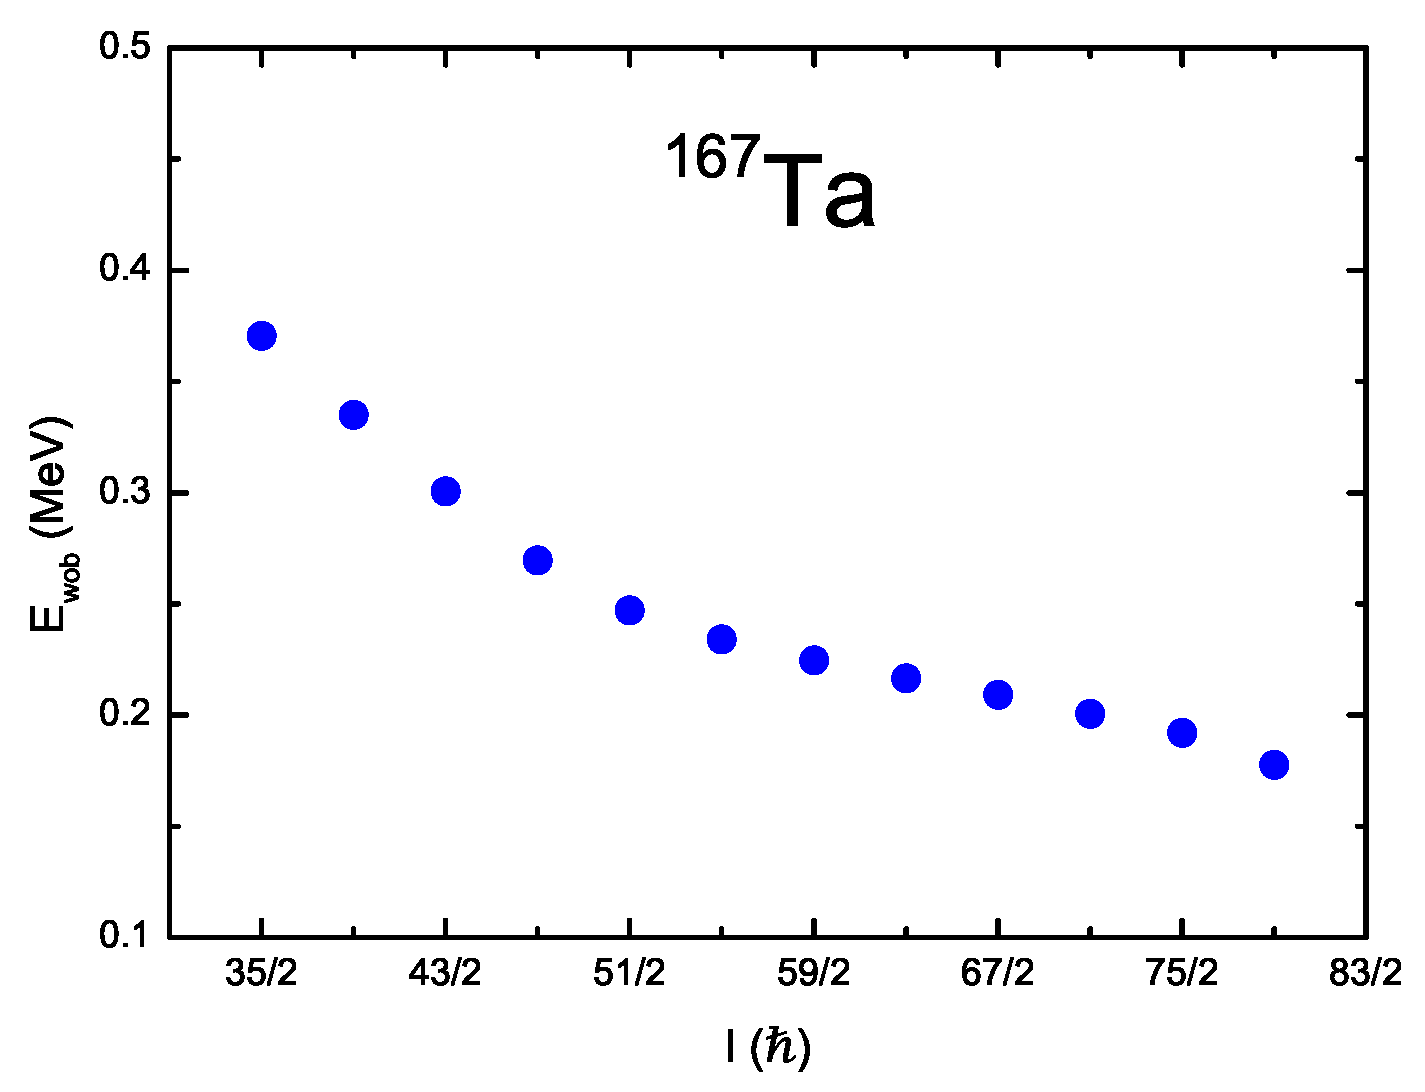
\includegraphics[height=0.25\textheight]{./img/c4/167Ta_plot.eps}}
	\caption{Wobbling frequencies of the $A\sim{}170$ wobblers. Top Left: $^{163}$Lu. Top Right: $^{165}$Lu. Middle Left: $^{167}$Lu. Middle Right: $^{161}$Lu. Bottom: $^{167}$Ta.\label{fig:chp4-old-wobb-freq}}
\end{figure}

To correct the deficiency in the QTR calculations of wobbling, S. Fraendorf and F. D\"onau introduced the concept of transverse and longitudinal wobbling \cite{frauendorfTransverseWobbling}. In this new scheme Refs. \cite{oldQTRWobblingTheory1,oldQTRWobblingTheory2,oldQTRWobblingTheory3,oldQTRWobblingTheory4} were describing longitudinal wobbling which is indeed expected to have an increasing wobbling frequency. A semi-classical analysis of transverse wobbling, which has the quasiparticle couple to an axis perpendicular to the intermediate axis, shows that the modified mode exhibits a decreasing wobbling frequency as has been seen in experimental observations of wobbling while reproducing the interband to intraband $B(E2)$ ratios.


\section{Triaxiality in the A$\sim$130 Region}
\label{sec:trw-triax}
Tr \cite{groundStateTriax}

\section{Level Scheme of $^{135}$Pr}
\label{sec:trw-lvl-scheme}

\subsection{Spin and Parity Assignments}
\label{ssec:trw-lvl-scheme-assignments}

\section{Description By Theory}
\label{sec:trw-theory-desc}

\section{Discussion}
\label{sec:trw-discussion}